% Diagrams for the Claude Code demo.
%
% Each tikzpicture below renders as its own cropped page thanks to
% \standaloneenv{tikzpicture}. Compile with:
%
%     pdflatex -interaction=nonstopmode diagrams.tex
%
% Output: diagrams.pdf, with one diagram per page. Convert to individual
% PNGs via:
%
%     pdftoppm -png -r 300 diagrams.pdf out
%
% Then drag the PNGs into the matching slides in Google Slides.

\documentclass[tikz,border=8pt]{standalone}
\usepackage{standalone}
\usepackage[T1]{fontenc}
\usepackage{helvet}
\renewcommand{\familydefault}{\sfdefault}
\usepackage{xcolor}
\usetikzlibrary{arrows.meta, positioning, shapes.geometric, fit, calc, backgrounds, shadows.blur, decorations.pathmorphing}

% One cropped page per tikzpicture.
\standaloneenv{tikzpicture}

% ------ color palette ------
\definecolor{navy}{HTML}{2C3E50}
\definecolor{blue}{HTML}{3498DB}
\definecolor{green}{HTML}{27AE60}
\definecolor{orange}{HTML}{E67E22}
\definecolor{red}{HTML}{E74C3C}
\definecolor{purple}{HTML}{9B59B6}
\definecolor{bg}{HTML}{F8F9FA}
\definecolor{softblue}{HTML}{EBF3FB}
\definecolor{softgreen}{HTML}{E8F5E8}
\definecolor{softorange}{HTML}{FDF2E3}
\definecolor{softred}{HTML}{FDECEA}
\definecolor{muted}{HTML}{7F8C8D}
\definecolor{code}{HTML}{F4F4F4}

% ------ common styles ------
\tikzset{
  box/.style={
    rectangle, rounded corners=3pt,
    draw=navy, fill=white, line width=0.8pt,
    minimum width=2.3cm, minimum height=1.1cm,
    align=center, font=\sffamily\small
  },
  softbox/.style={box, fill=softblue, draw=blue!70},
  greenbox/.style={box, fill=softgreen, draw=green!70},
  orangebox/.style={box, fill=softorange, draw=orange!70},
  redbox/.style={box, fill=softred, draw=red!70},
  darkbox/.style={box, fill=navy, draw=navy, text=white},
  label/.style={font=\sffamily\footnotesize\itshape, text=muted, align=center},
  arrow/.style={-{Latex[length=2.5mm,width=2mm]}, line width=0.7pt, draw=navy!80},
  bigarrow/.style={-{Latex[length=3.5mm,width=3mm]}, line width=1.2pt, draw=navy},
  broken/.style={decorate, decoration={zigzag, segment length=4pt, amplitude=1.5pt},
                 line width=1pt, draw=red},
}

\begin{document}

% =========================================================================
% 1. MEMORY — Claude with 4 markdown files around it
% =========================================================================
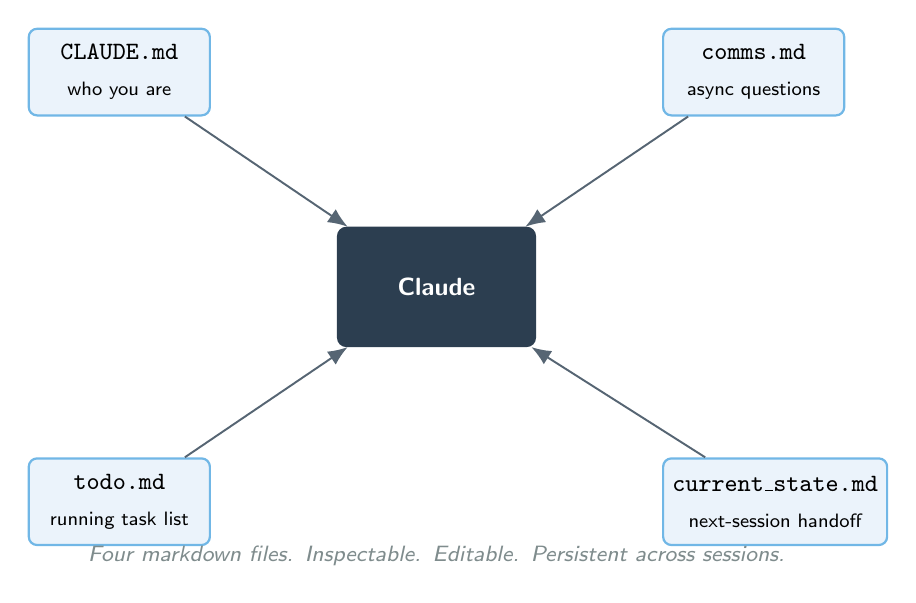
\begin{tikzpicture}[node distance=1.8cm]
  \node[darkbox, minimum width=2.5cm, minimum height=1.5cm] (claude) at (0,0)
    {\bfseries Claude};

  \node[softbox, above left=1.4cm and 1.6cm of claude]
    (cmd) {\ttfamily CLAUDE.md\\[2pt]\normalfont\scriptsize who you are};
  \node[softbox, above right=1.4cm and 1.6cm of claude]
    (comms) {\ttfamily comms.md\\[2pt]\normalfont\scriptsize async questions};
  \node[softbox, below left=1.4cm and 1.6cm of claude]
    (todo) {\ttfamily todo.md\\[2pt]\normalfont\scriptsize running task list};
  \node[softbox, below right=1.4cm and 1.6cm of claude]
    (state) {\ttfamily current\_state.md\\[2pt]\normalfont\scriptsize next-session handoff};

  \draw[arrow] (cmd) -- (claude);
  \draw[arrow] (comms) -- (claude);
  \draw[arrow] (todo) -- (claude);
  \draw[arrow] (state) -- (claude);

  \node[label, below=2.4cm of claude, text width=10cm]
    {Four markdown files. Inspectable. Editable. Persistent across sessions.};
\end{tikzpicture}

% =========================================================================
% 2. JOKE_FLOW — 6 boxes left to right
% =========================================================================
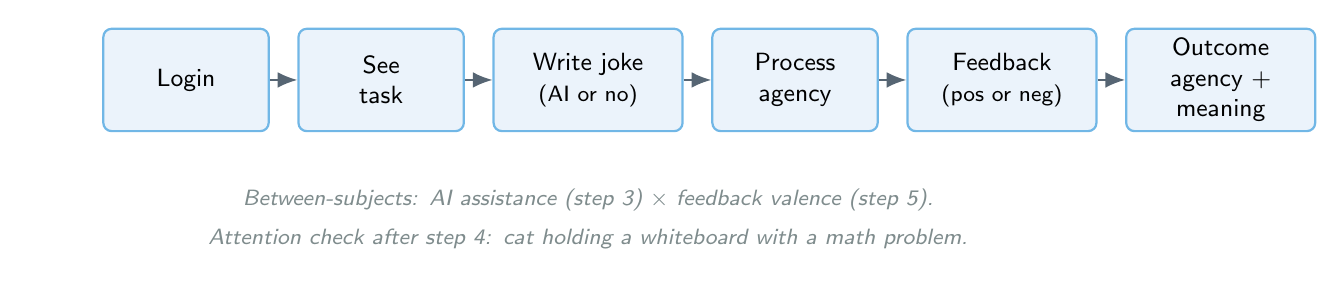
\begin{tikzpicture}[node distance=0.35cm]
  \node[softbox, minimum width=2.1cm, minimum height=1.3cm] (s1) {Login};
  \node[softbox, right=of s1, minimum width=2.1cm, minimum height=1.3cm] (s2) {See\\task};
  \node[softbox, right=of s2, minimum width=2.4cm, minimum height=1.3cm] (s3) {Write joke\\\footnotesize{(AI or no)}};
  \node[softbox, right=of s3, minimum width=2.1cm, minimum height=1.3cm] (s4) {Process\\agency};
  \node[softbox, right=of s4, minimum width=2.4cm, minimum height=1.3cm] (s5) {Feedback\\\footnotesize{(pos or neg)}};
  \node[softbox, right=of s5, minimum width=2.4cm, minimum height=1.3cm] (s6) {Outcome\\agency +\\meaning};

  \foreach \from/\to in {s1/s2, s2/s3, s3/s4, s4/s5, s5/s6}
    \draw[arrow] (\from) -- (\to);

  \node[label, below=0.6cm of s3, text width=14cm]
    {Between-subjects: AI assistance (step 3) $\times$ feedback valence (step 5).};
  \node[label, below=1.1cm of s3, text width=14cm, text=muted]
    {Attention check after step 4: cat holding a whiteboard with a math problem.};
\end{tikzpicture}

% =========================================================================
% 3. COMMIT_HASH — materials + data both tied to git SHA
% =========================================================================
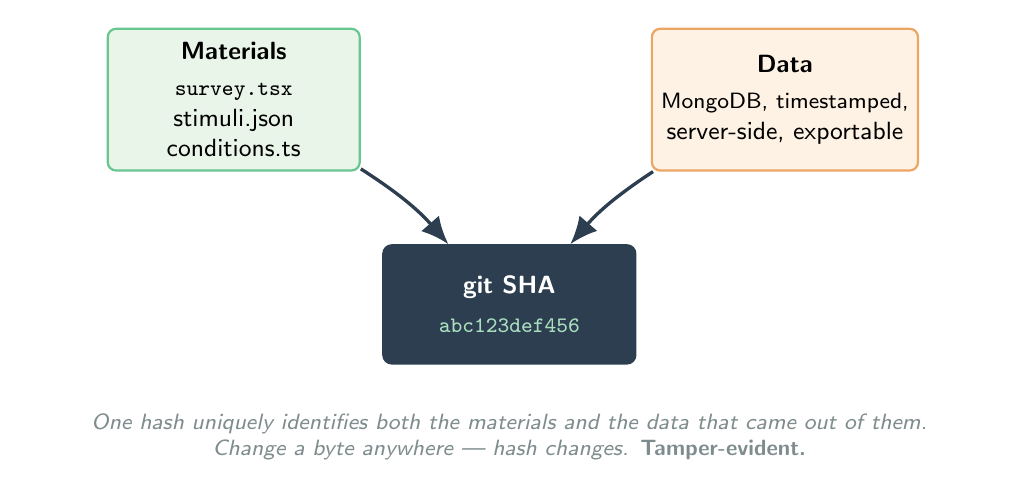
\begin{tikzpicture}
  \node[greenbox, minimum width=3.2cm, minimum height=1.8cm] (mat) at (-3.5, 1.2)
    {\bfseries Materials\\[2pt]\normalfont\footnotesize\ttfamily survey.tsx\\stimuli.json\\conditions.ts};
  \node[orangebox, minimum width=3.2cm, minimum height=1.8cm] (data) at (3.5, 1.2)
    {\bfseries Data\\[2pt]\normalfont\footnotesize MongoDB, timestamped,\\server-side, exportable};
  \node[darkbox, minimum width=3.2cm, minimum height=1.5cm] (sha) at (0, -1.4)
    {\bfseries git SHA\\[3pt]\normalfont\ttfamily\footnotesize\textcolor{green!40!white}{abc123def456}};

  \draw[bigarrow] (mat) to[bend left=8] (sha);
  \draw[bigarrow] (data) to[bend right=8] (sha);

  \node[label, below=0.5cm of sha, text width=12cm]
    {One hash uniquely identifies both the materials and the data that came out of them.\\
     Change a byte anywhere --- hash changes. \textbf{Tamper-evident.}};
\end{tikzpicture}

% =========================================================================
% 4. WEBAPP_ARCH — React → Express → MongoDB
% =========================================================================
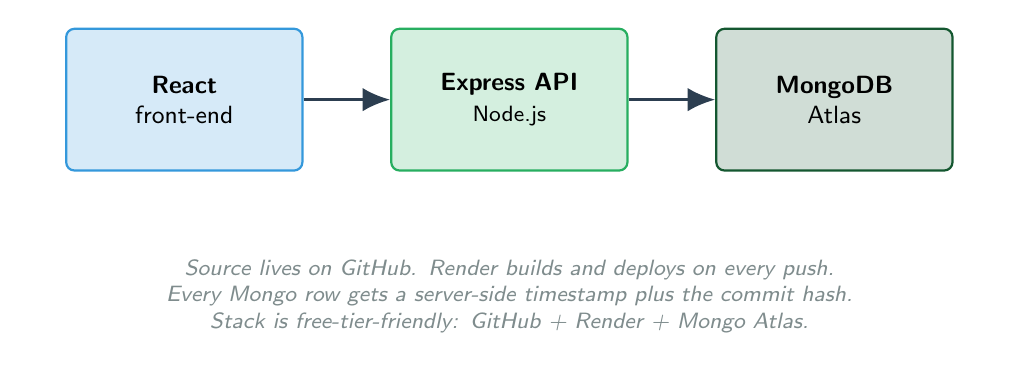
\begin{tikzpicture}[node distance=1.1cm]
  \node[box, fill=blue!20, draw=blue, minimum width=3cm, minimum height=1.8cm] (react)
    {\bfseries React\\front-end};
  \node[box, fill=green!20, draw=green, right=of react, minimum width=3cm, minimum height=1.8cm] (api)
    {\bfseries Express API\\{\footnotesize Node.js}};
  \node[box, fill=green!50!black!20, draw=green!50!black, right=of api, minimum width=3cm, minimum height=1.8cm] (mongo)
    {\bfseries MongoDB\\Atlas};

  \draw[bigarrow] (react) -- (api);
  \draw[bigarrow] (api) -- (mongo);

  \node[label, below=1cm of api, text width=12cm]
    {Source lives on GitHub. Render builds and deploys on every push.\\
     Every Mongo row gets a server-side timestamp plus the commit hash.\\
     Stack is free-tier-friendly: GitHub + Render + Mongo Atlas.};
\end{tikzpicture}

% =========================================================================
% 5. QMD_CASCADE — one literate document, top to bottom
% =========================================================================
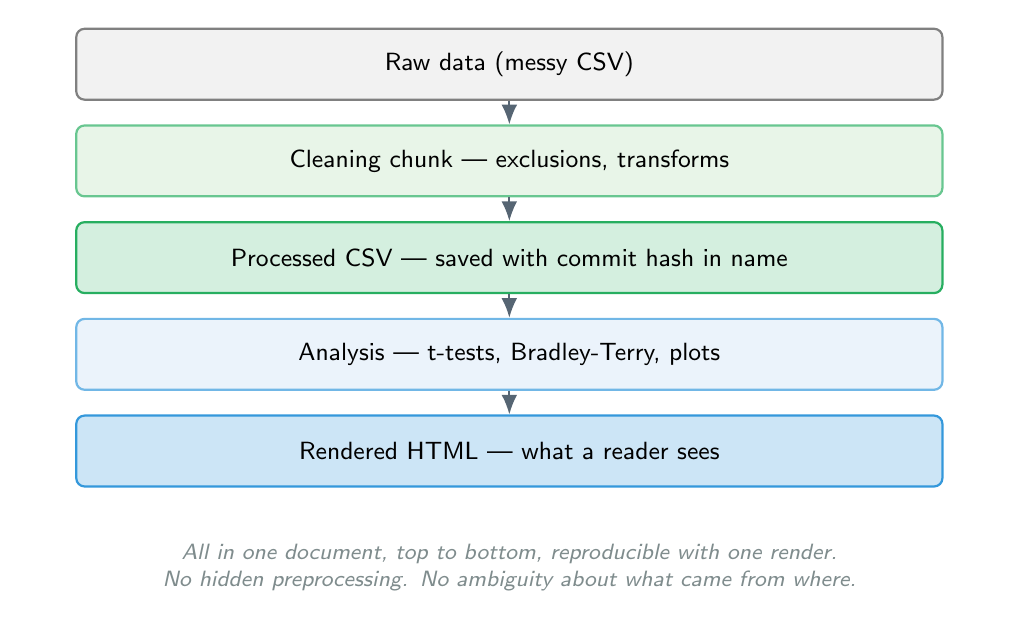
\begin{tikzpicture}[node distance=0.3cm]
  \node[box, fill=gray!10, draw=gray, minimum width=11cm, minimum height=0.9cm] (raw)
    {Raw data (messy CSV)};
  \node[box, fill=softgreen, draw=green!70, below=of raw, minimum width=11cm, minimum height=0.9cm] (clean)
    {Cleaning chunk --- exclusions, transforms};
  \node[box, fill=green!20, draw=green, below=of clean, minimum width=11cm, minimum height=0.9cm] (csv)
    {Processed CSV --- saved with commit hash in name};
  \node[box, fill=softblue, draw=blue!70, below=of csv, minimum width=11cm, minimum height=0.9cm] (analysis)
    {Analysis --- t-tests, Bradley-Terry, plots};
  \node[box, fill=blue!25, draw=blue, below=of analysis, minimum width=11cm, minimum height=0.9cm] (html)
    {Rendered HTML --- what a reader sees};

  \foreach \from/\to in {raw/clean, clean/csv, csv/analysis, analysis/html}
    \draw[arrow] (\from) -- (\to);

  \node[label, below=0.6cm of html, text width=12cm]
    {All in one document, top to bottom, reproducible with one render.\\
     No hidden preprocessing. No ambiguity about what came from where.};
\end{tikzpicture}

% =========================================================================
% 6. NO_MAGIC — code and manuscript linked
% =========================================================================
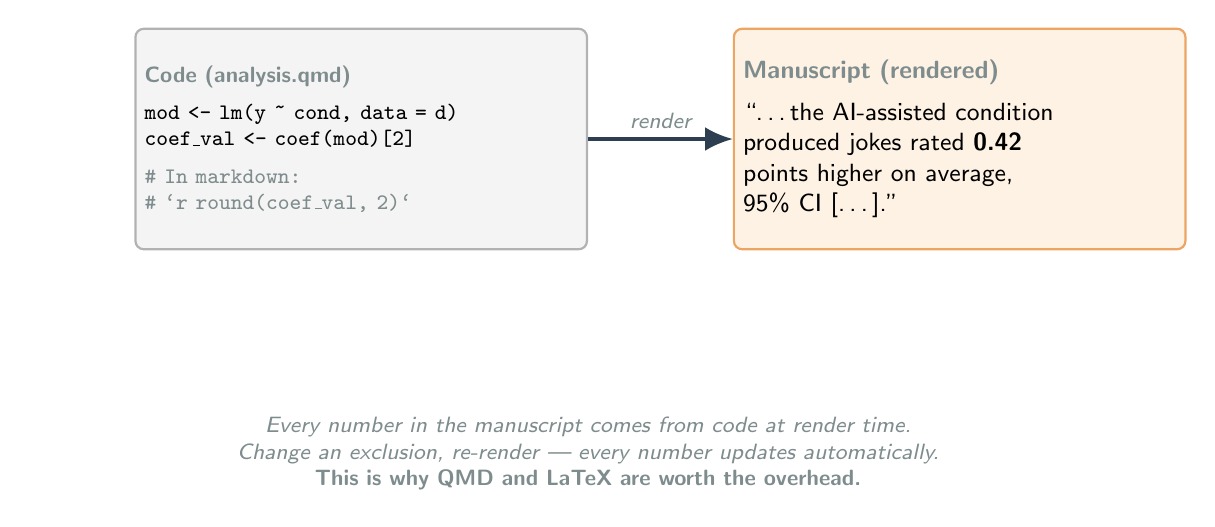
\begin{tikzpicture}
  \node[box, fill=code, draw=gray!60, text width=5.5cm, minimum height=2.8cm, align=left, font=\ttfamily\footnotesize] (code) at (-3.8,0) {
    \textcolor{muted}{\sffamily\bfseries Code (analysis.qmd)}\\[4pt]
    mod <- lm(y \~{}\ cond, data = d)\\
    coef\_val <- coef(mod)[2]\\[4pt]
    \textcolor{muted}{\# In markdown:}\\
    \textcolor{muted}{\# `r round(coef\_val, 2)`}
  };

  \node[box, fill=softorange, draw=orange!70, text width=5.5cm, minimum height=2.8cm, align=left] (ms) at (3.8,0) {
    \textcolor{muted}{\bfseries Manuscript (rendered)}\\[4pt]
    ``\ldots the AI-assisted condition\\produced jokes rated \textbf{0.42}\\points higher on average,\\95\% CI [\ldots].''
  };

  \draw[bigarrow] (code) -- (ms) node[midway, above, label] {render};

  \node[label, below=2.0cm of code.south east, anchor=north, text width=14cm]
    {Every number in the manuscript comes from code at render time.\\
     Change an exclusion, re-render --- every number updates automatically.\\
     \textbf{This is why QMD and LaTeX are worth the overhead.}};
\end{tikzpicture}

% =========================================================================
% 7. GDOCS_TRAP — broken link after export to Google Docs
% =========================================================================
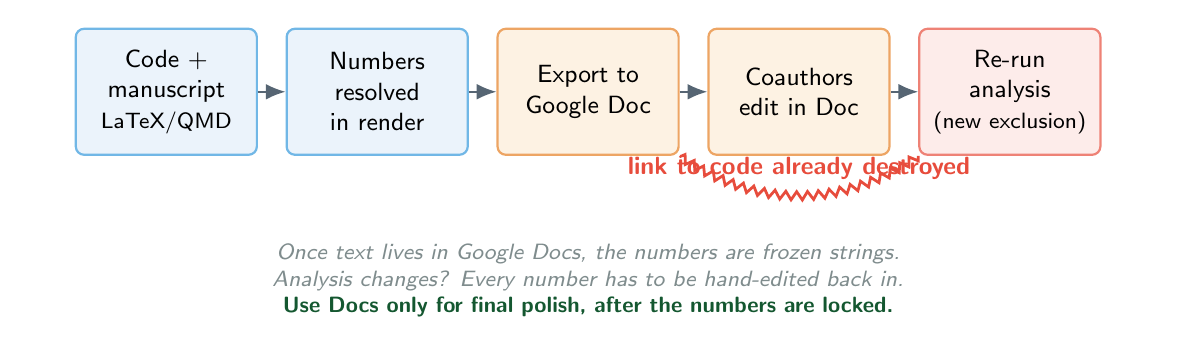
\begin{tikzpicture}[node distance=0.35cm]
  \node[softbox, minimum width=2.3cm, minimum height=1.6cm] (a) {Code +\\manuscript\\{\footnotesize LaTeX/QMD}};
  \node[softbox, right=of a, minimum width=2.3cm, minimum height=1.6cm] (b) {Numbers\\resolved\\in render};
  \node[orangebox, right=of b, minimum width=2.3cm, minimum height=1.6cm] (c) {Export to\\Google Doc};
  \node[orangebox, right=of c, minimum width=2.3cm, minimum height=1.6cm] (d) {Coauthors\\edit in Doc};
  \node[redbox, right=of d, minimum width=2.3cm, minimum height=1.6cm] (e) {Re-run\\analysis\\{\footnotesize (new exclusion)}};

  \draw[arrow] (a) -- (b);
  \draw[arrow] (b) -- (c);
  \draw[arrow] (c) -- (d);
  \draw[arrow] (d) -- (e);

  % Attempt to feed results back — broken
  \draw[broken] (e) to[bend left=35] node[above, label, yshift=2pt] {\textcolor{red}{\bfseries\small link to code already destroyed}} (c);

  \node[label, below=1cm of c, text width=14cm]
    {Once text lives in Google Docs, the numbers are frozen strings.\\
     Analysis changes? Every number has to be hand-edited back in.\\
     \textbf{\textcolor{green!50!black}{Use Docs only for final polish, after the numbers are locked.}}};
\end{tikzpicture}

% =========================================================================
% 8. OVERLEAF_FLOW — 4-box loop
% =========================================================================
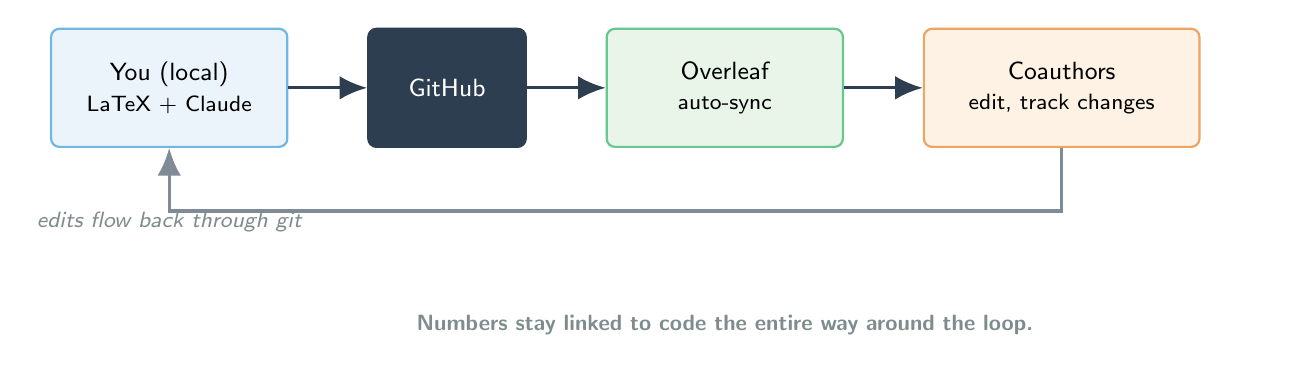
\begin{tikzpicture}[node distance=1.0cm]
  \node[softbox, minimum width=3cm, minimum height=1.5cm] (you) {You (local)\\{\footnotesize LaTeX + Claude}};
  \node[darkbox, right=of you, minimum width=2cm, minimum height=1.5cm] (github) {GitHub};
  \node[greenbox, right=of github, minimum width=3cm, minimum height=1.5cm] (overleaf) {Overleaf\\{\footnotesize auto-sync}};
  \node[softbox, right=of overleaf, fill=softorange, draw=orange!70, minimum width=3.5cm, minimum height=1.5cm] (co) {Coauthors\\{\footnotesize edit, track changes}};

  \draw[bigarrow] (you) -- (github);
  \draw[bigarrow] (github) -- (overleaf);
  \draw[bigarrow] (overleaf) -- (co);

  % return loop
  \coordinate (below-co) at ($(co.south) + (0,-0.8cm)$);
  \coordinate (below-you) at ($(you.south) + (0,-0.8cm)$);
  \draw[bigarrow, draw=navy!60]
    (co.south) -- (below-co)
    -- (below-you) -- (you.south)
    node[midway, above, label, yshift=-0.8cm] {edits flow back through git};

  \node[label, below=2.0cm of overleaf, text width=14cm]
    {\textbf{Numbers stay linked to code the entire way around the loop.}};
\end{tikzpicture}

% =========================================================================
% 9. PROVENANCE — Prolific → Mongo → git SHA
% =========================================================================
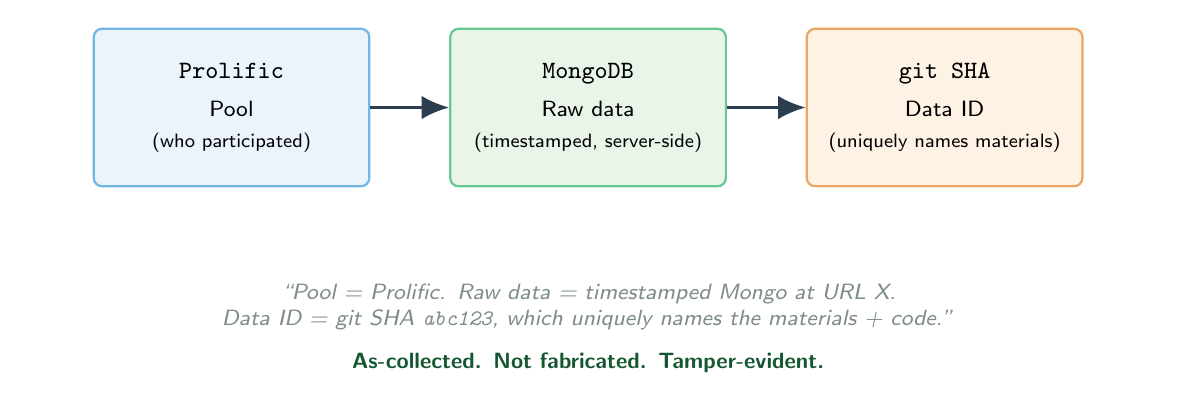
\begin{tikzpicture}[node distance=1.0cm]
  \node[softbox, minimum width=3.5cm, minimum height=2.0cm] (pool)
    {\bfseries\ttfamily Prolific\\[3pt]\normalfont\footnotesize Pool\\{\scriptsize (who participated)}};
  \node[greenbox, right=of pool, minimum width=3.5cm, minimum height=2.0cm] (mongo)
    {\bfseries\ttfamily MongoDB\\[3pt]\normalfont\footnotesize Raw data\\{\scriptsize (timestamped, server-side)}};
  \node[orangebox, right=of mongo, minimum width=3.5cm, minimum height=2.0cm] (sha)
    {\bfseries\ttfamily git SHA\\[3pt]\normalfont\footnotesize Data ID\\{\scriptsize (uniquely names materials)}};

  \draw[bigarrow] (pool) -- (mongo);
  \draw[bigarrow] (mongo) -- (sha);

  \node[label, below=1.1cm of mongo, text width=14cm, align=center]
    {``Pool = Prolific. Raw data = timestamped Mongo at URL X.\\
     Data ID = git SHA \texttt{abc123}, which uniquely names the materials + code.''\\[6pt]
     \textbf{\textcolor{green!50!black}{As-collected. Not fabricated. Tamper-evident.}}};
\end{tikzpicture}

\end{document}
